\chapter{Spectrum Analyzer}
The specific target of this exploit, is the tool called the spectrum analyzer, which can be exploited through a buffer overflow.
The intended purpose of the spectrum analyzer is to identify potential problems with the connection through the cable, such as interference.
The spectrum analyzer is exposed to the local network, although on varying ports depending on particular cable modem.
It can usually be discovered by running NMAP on \mono{192.168.100.*}, see \cref{lst:nmap_command}, which redirects to the modem itself, often either on \mono{192.168.0.1} or \mono{192.168.1.1}.
In some cases the endpoint require credentials, but so far a default set has been seen working on every example, as shown in \appendixref{app:ExploredRouters}.

\begin{lstlisting}[language=sh,firstnumber=1,label={lst:nmap_command},caption={The NMAP request to find the Spectrum Analyser},float]
    nmap 192.168.100.0/24
\end{lstlisting}

\section{Overflowing the Registers}
Requests to the spectrum analyzer is sent as JSON through a websocket. An example of an intended request can be seen in \cref{lst:json_intended}.
\lstinputlisting[language=json,firstnumber=1,label={lst:json_intended},caption={An expected request.},float]{legit_request.json}

However, the JSON deserializer used in the spectrum analyzer, allocates a predefined amount of memory for each parameter, but will keep reading input parameters until a comma (,) is reached.
This can be exploited with a malicious request, like the one seen in \cref{lst:json_malicious}.
Here the fStartHz has a parameter value bigger than the allocated memory, and will therefore overflow and overwrite the registers.
To validate this, a json package with 200 A's as the fStartHz parameter can be sent through the serial port to the CM.
This will crash the modem and all register values will be displayed, showing that the program counter has changed to 0x41414141.
A more thorough walk-through of how to check this, is given in \appendixref{app:howto}.

\lstinputlisting[language=json,firstnumber=1,label={lst:json_malicious},caption={A malicious request.},float]{overflow_request.json}


\section{Return Oriented Programming}
The CM architecture saves callee registers on the stack and restores these before returning. 
Therefore, if we overwrite the variable registers S0-S7 and the return address register saved on the stack, we can run any existing code in the system, with our desired input variables.
Although we are not able to execute our own code yet, through return oriented programming we are able to execute existing code on the system in a turing-complete manner and manipulate the system extensively.
This can be used to open a telnet server for external root access to the CM, allowing remote access to the system.
Through this telnet we can access a range of methods, but most importantly we can read and write memory addresses, and execute code from any memory address, including ones we have just written to.
These last steps varies from modem to modem, but one complete example can be found in \appendixref{app:technical_replication}.

% \begin{figure}
%   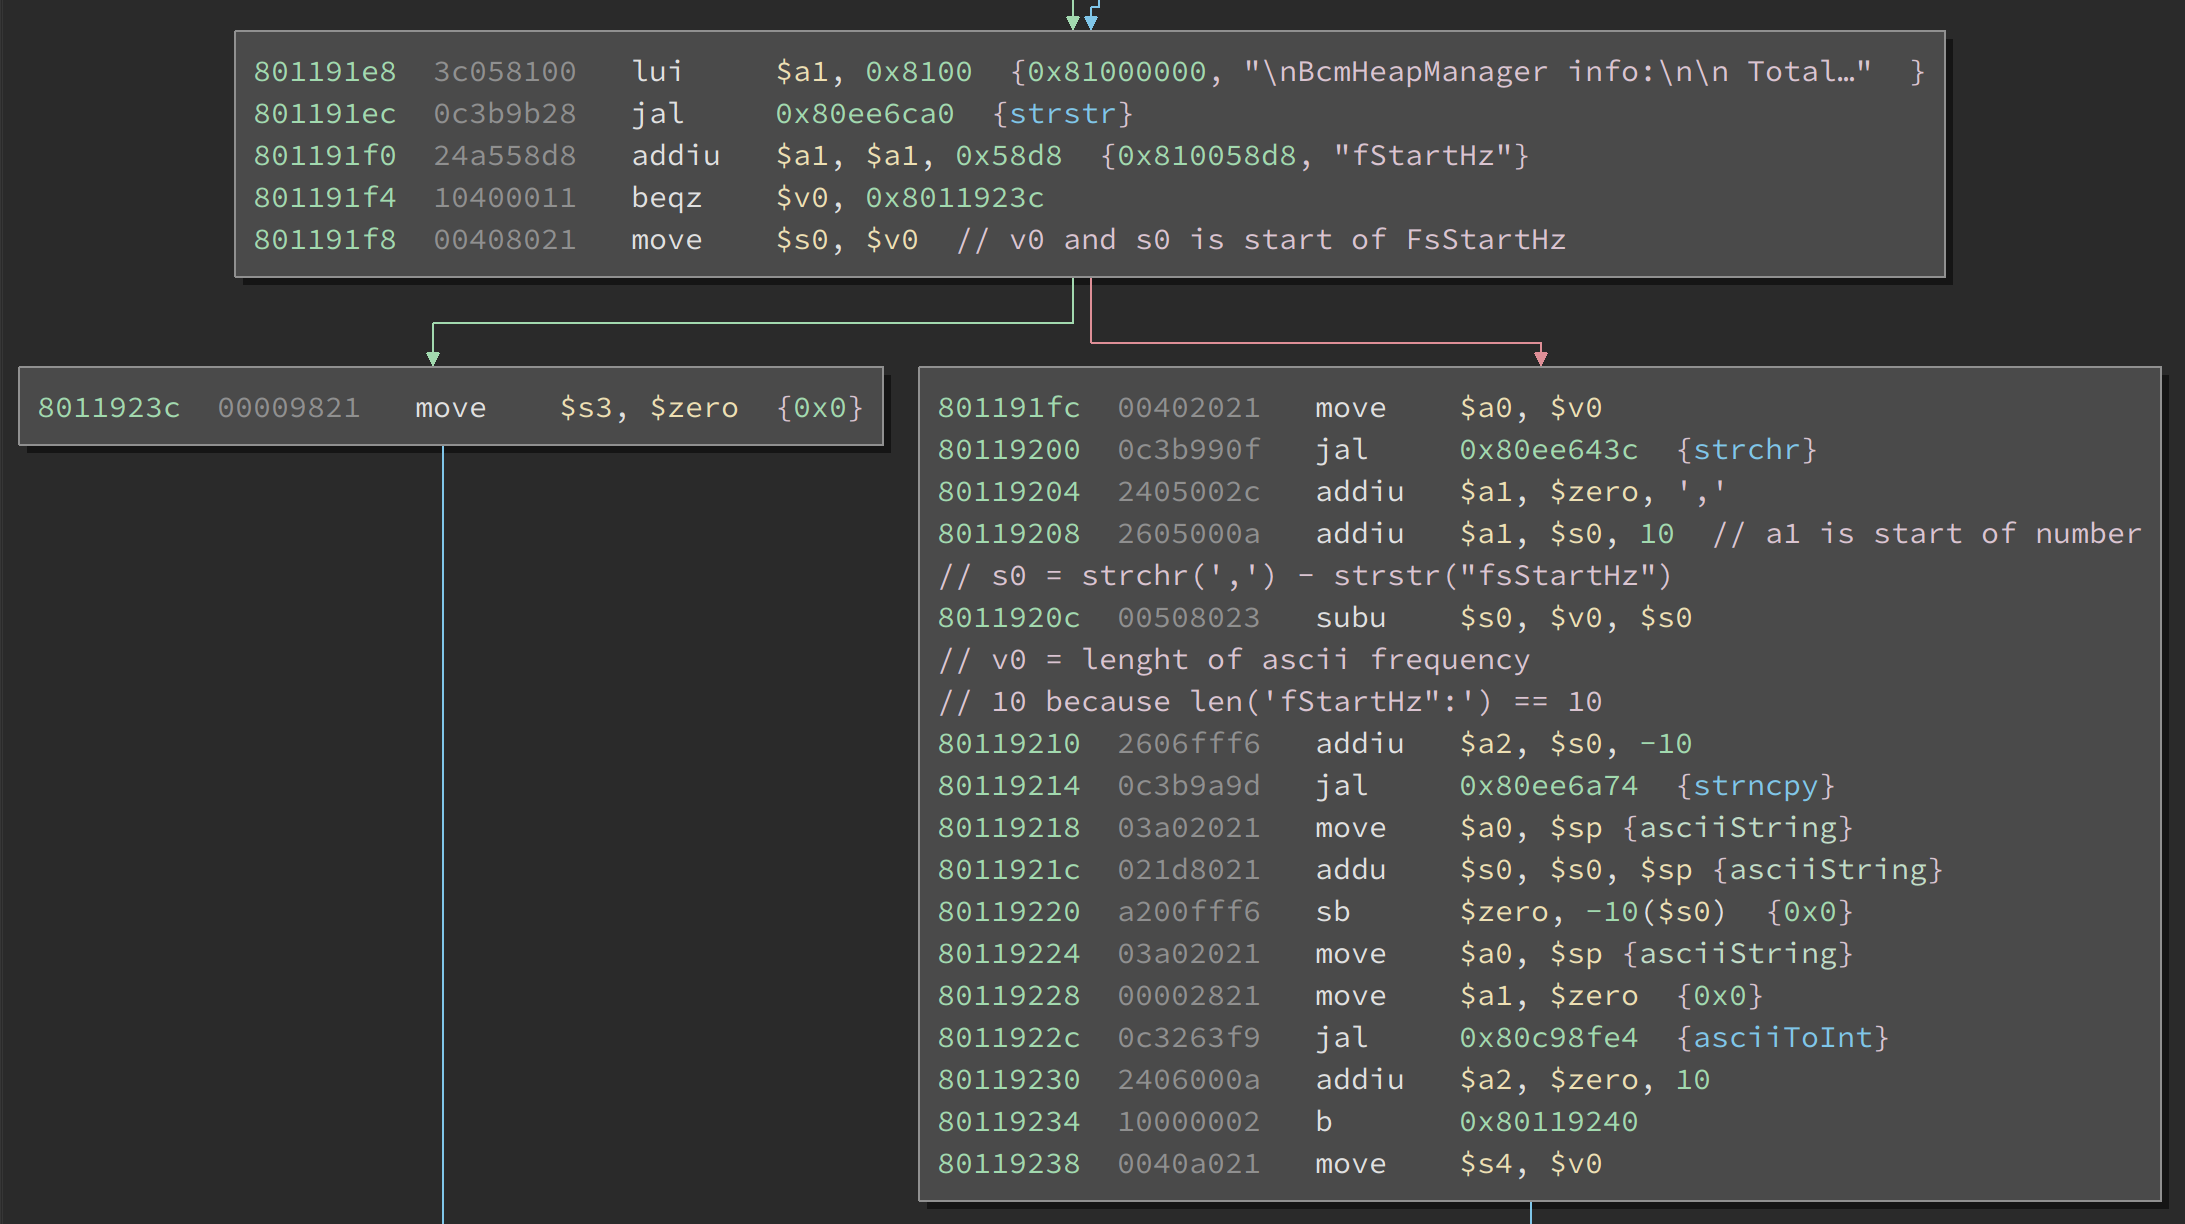
\includegraphics[width=\linewidth]{../graphics/spectrum.png}
%   \caption{Buffer overflow in beginning of stack as strncpy copies until it reaches a comma}
%   \label{fig:spectrum}
% \end{figure}
